\subsection{Durchflussmessung}
\label{subsec:Durchflussmessung}

Da gemäss Kapitel \ref{subsubsec:Pumpen} Pumpen eingesetzt werden, welche nicht über eine integrierte Durchflussmessung verfügen, muss diese extern gemessen werden. Dies wird mittels Durchflusssensoren umgesetzt. Dazu werden verschiedene Möglichkeiten verglichen.

\subsubsection{Anforderungen}\label{par:Anforderungen_Durchflussmessung}

\begin{tabularx}{\textwidth}{lllX}
Durchflussmenge & : & Aus Pflichtziel & min. 0.6l pro Minute\\
 & & Aus Wunschziel & min 1.2l pro Minute \\
Spannung & : & Spannungsversorgung & 3.3V bis 5V \\
Schlauchanschluss & : & Innendurchmesser & 6-8mm \\
Sonstiges & : & Hygieneanforderungen & Lebensmittelsensor \\
\end{tabularx}

Es existieren viele verschiedene Varianten um eine Durchflussmessung durchführen zu können. Dazu gehören folgende Verfahren:

\begin{itemize}
\item akustische Verfahren
\item gyroskopische Verfahren
\item magnetisch-induktive Verfahren
\item mechanisch-volumetrische Verfahren
\item optische Verfahren
\item thermische Verfahren
\item Wirkdruck-/Stauverfahren
\end{itemize}

Viele dieser Verfahren werden nur bei grösseren Durchflussmengen eingesetzt. Wieder andere werden verwendet um den Durchfluss von verschieden Medien zu bemessen. Da es sich bei diesem Projekt um relativ geringe Durchflussmengen von weniger als 2l/min handelt eignet sich ein mechanisch-volumetrisches Verfahren am besten. \cite{alfaomega_durchflussmesser_2019}

\subsubsection{Verwendeter Durchflusssensor}\label{par:Verwendter_Durchflussssensor}

Beim verwendeten Durchflussmessgerät handelt es sich um ein sogenannten Flügelradzähler von Sea gemäss Abbildung \ref{fig:Flügelradzähler}. Dies ist ein hermetisch abgeschlossener Durchflussgeber, dessen Kernstück aus einem Flügelrad besteht. Bei Durchfluss wird dieses Flügelrad in Bewegung gesetzt, welches über einen Hallsensor elektronische Impulse erzeugt. Somit kann die durchfliessende Menge elektronisch bestimmt werden. \cite{five_+_tools_store_us_nodate}
 
\begin{figure}[h!]
	\centering
	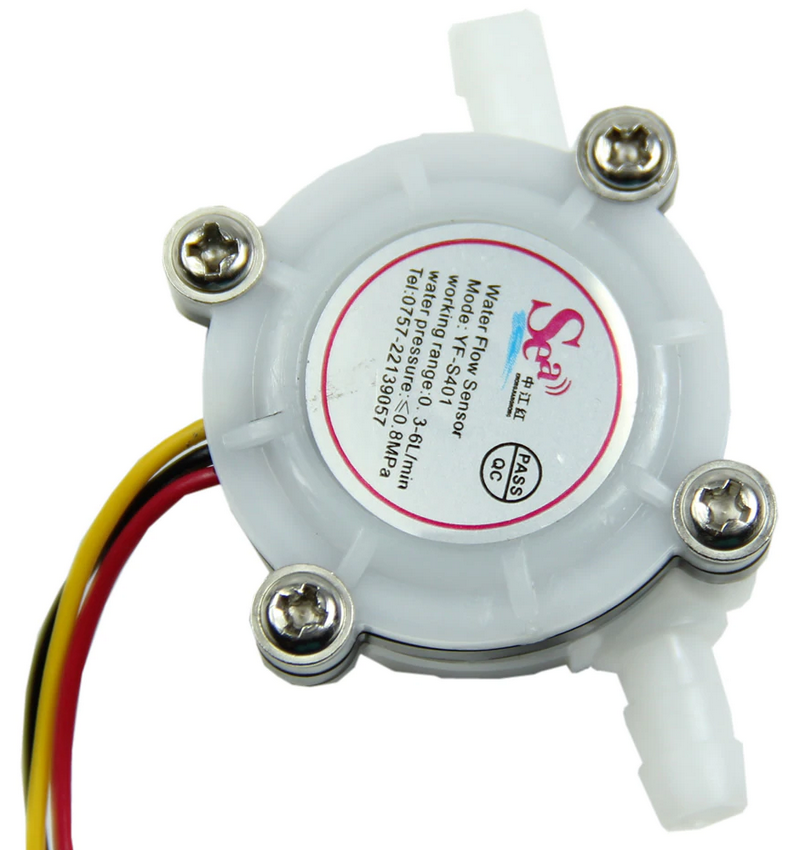
\includegraphics[width=0.6\textwidth]{graphics/Fluegelradzaehler.png}
	\caption{Sea Flügelradzähler \cite{five_+_tools_store_us_nodate}}
	\label{fig:Flügelradzähler}
\end{figure}

\begin{table}[h!]
\centering
\begin{tabularx}{\textwidth/2}{|X|}
\hline
\textbf{Technische Daten:}\\
\hline
- Spannung: 3.3 - 5V\\

- Sromverbrauch: ca. 15mA\\

- Messbarere Durchflussmenge: 0.3-6l/min\\

- Preis: 2.09 CHF \\

- Bestellseite: Aliexpress\\

\hline
\end{tabularx}
\caption{Technische Daten Sea Durchflussmessgerät \cite{five_+_tools_store_us_nodate}}
\end{table}
